\documentclass[11pt,a4paper,]{article}
\usepackage{lmodern}

\usepackage{amssymb,amsmath}
\usepackage{ifxetex,ifluatex}
\usepackage{fixltx2e} % provides \textsubscript
\ifnum 0\ifxetex 1\fi\ifluatex 1\fi=0 % if pdftex
  \usepackage[T1]{fontenc}
  \usepackage[utf8]{inputenc}
\else % if luatex or xelatex
  \usepackage{unicode-math}
  \defaultfontfeatures{Ligatures=TeX,Scale=MatchLowercase}
\fi
% use upquote if available, for straight quotes in verbatim environments
\IfFileExists{upquote.sty}{\usepackage{upquote}}{}
% use microtype if available
\IfFileExists{microtype.sty}{%
\usepackage[]{microtype}
\UseMicrotypeSet[protrusion]{basicmath} % disable protrusion for tt fonts
}{}
\PassOptionsToPackage{hyphens}{url} % url is loaded by hyperref
\usepackage[unicode=true]{hyperref}
\hypersetup{
            pdftitle={Crime in Minneapolis},
            pdfborder={0 0 0},
            breaklinks=true}
\urlstyle{same}  % don't use monospace font for urls
\usepackage{geometry}
\geometry{a4paper, centering, text={16cm,24cm}}
\usepackage[style=authoryear-comp,]{biblatex}
\addbibresource{references.bib}
\usepackage{color}
\usepackage{fancyvrb}
\newcommand{\VerbBar}{|}
\newcommand{\VERB}{\Verb[commandchars=\\\{\}]}
\DefineVerbatimEnvironment{Highlighting}{Verbatim}{commandchars=\\\{\}}
% Add ',fontsize=\small' for more characters per line
\usepackage{framed}
\definecolor{shadecolor}{RGB}{248,248,248}
\newenvironment{Shaded}{\begin{snugshade}}{\end{snugshade}}
\newcommand{\AlertTok}[1]{\textcolor[rgb]{0.94,0.16,0.16}{#1}}
\newcommand{\AnnotationTok}[1]{\textcolor[rgb]{0.56,0.35,0.01}{\textbf{\textit{#1}}}}
\newcommand{\AttributeTok}[1]{\textcolor[rgb]{0.77,0.63,0.00}{#1}}
\newcommand{\BaseNTok}[1]{\textcolor[rgb]{0.00,0.00,0.81}{#1}}
\newcommand{\BuiltInTok}[1]{#1}
\newcommand{\CharTok}[1]{\textcolor[rgb]{0.31,0.60,0.02}{#1}}
\newcommand{\CommentTok}[1]{\textcolor[rgb]{0.56,0.35,0.01}{\textit{#1}}}
\newcommand{\CommentVarTok}[1]{\textcolor[rgb]{0.56,0.35,0.01}{\textbf{\textit{#1}}}}
\newcommand{\ConstantTok}[1]{\textcolor[rgb]{0.00,0.00,0.00}{#1}}
\newcommand{\ControlFlowTok}[1]{\textcolor[rgb]{0.13,0.29,0.53}{\textbf{#1}}}
\newcommand{\DataTypeTok}[1]{\textcolor[rgb]{0.13,0.29,0.53}{#1}}
\newcommand{\DecValTok}[1]{\textcolor[rgb]{0.00,0.00,0.81}{#1}}
\newcommand{\DocumentationTok}[1]{\textcolor[rgb]{0.56,0.35,0.01}{\textbf{\textit{#1}}}}
\newcommand{\ErrorTok}[1]{\textcolor[rgb]{0.64,0.00,0.00}{\textbf{#1}}}
\newcommand{\ExtensionTok}[1]{#1}
\newcommand{\FloatTok}[1]{\textcolor[rgb]{0.00,0.00,0.81}{#1}}
\newcommand{\FunctionTok}[1]{\textcolor[rgb]{0.00,0.00,0.00}{#1}}
\newcommand{\ImportTok}[1]{#1}
\newcommand{\InformationTok}[1]{\textcolor[rgb]{0.56,0.35,0.01}{\textbf{\textit{#1}}}}
\newcommand{\KeywordTok}[1]{\textcolor[rgb]{0.13,0.29,0.53}{\textbf{#1}}}
\newcommand{\NormalTok}[1]{#1}
\newcommand{\OperatorTok}[1]{\textcolor[rgb]{0.81,0.36,0.00}{\textbf{#1}}}
\newcommand{\OtherTok}[1]{\textcolor[rgb]{0.56,0.35,0.01}{#1}}
\newcommand{\PreprocessorTok}[1]{\textcolor[rgb]{0.56,0.35,0.01}{\textit{#1}}}
\newcommand{\RegionMarkerTok}[1]{#1}
\newcommand{\SpecialCharTok}[1]{\textcolor[rgb]{0.00,0.00,0.00}{#1}}
\newcommand{\SpecialStringTok}[1]{\textcolor[rgb]{0.31,0.60,0.02}{#1}}
\newcommand{\StringTok}[1]{\textcolor[rgb]{0.31,0.60,0.02}{#1}}
\newcommand{\VariableTok}[1]{\textcolor[rgb]{0.00,0.00,0.00}{#1}}
\newcommand{\VerbatimStringTok}[1]{\textcolor[rgb]{0.31,0.60,0.02}{#1}}
\newcommand{\WarningTok}[1]{\textcolor[rgb]{0.56,0.35,0.01}{\textbf{\textit{#1}}}}
\usepackage{longtable,booktabs}
% Fix footnotes in tables (requires footnote package)
\IfFileExists{footnote.sty}{\usepackage{footnote}\makesavenoteenv{long table}}{}
\usepackage{graphicx,grffile}
\makeatletter
\def\maxwidth{\ifdim\Gin@nat@width>\linewidth\linewidth\else\Gin@nat@width\fi}
\def\maxheight{\ifdim\Gin@nat@height>\textheight\textheight\else\Gin@nat@height\fi}
\makeatother
% Scale images if necessary, so that they will not overflow the page
% margins by default, and it is still possible to overwrite the defaults
% using explicit options in \includegraphics[width, height, ...]{}
\setkeys{Gin}{width=\maxwidth,height=\maxheight,keepaspectratio}
\IfFileExists{parskip.sty}{%
\usepackage{parskip}
}{% else
\setlength{\parindent}{0pt}
\setlength{\parskip}{6pt plus 2pt minus 1pt}
}
\setlength{\emergencystretch}{3em}  % prevent overfull lines
\providecommand{\tightlist}{%
  \setlength{\itemsep}{0pt}\setlength{\parskip}{0pt}}
\setcounter{secnumdepth}{5}

% set default figure placement to htbp
\makeatletter
\def\fps@figure{htbp}
\makeatother


\title{Crime in Minneapolis}

%% MONASH STUFF

%% CAPTIONS
\RequirePackage{caption}
\DeclareCaptionStyle{italic}[justification=centering]
 {labelfont={bf},textfont={it},labelsep=colon}
\captionsetup[figure]{style=italic,format=hang,singlelinecheck=true}
\captionsetup[table]{style=italic,format=hang,singlelinecheck=true}


%% FONT
\RequirePackage{bera}
\RequirePackage[charter,expert,sfscaled]{mathdesign}
\RequirePackage{fontawesome}

%% HEADERS AND FOOTERS
\RequirePackage{fancyhdr}
\pagestyle{fancy}
\rfoot{\Large\sffamily\raisebox{-0.1cm}{\textbf{\thepage}}}
\makeatletter
\lhead{\textsf{\expandafter{\@title}}}
\makeatother
\rhead{}
\cfoot{}
\setlength{\headheight}{15pt}
\renewcommand{\headrulewidth}{0.4pt}
\renewcommand{\footrulewidth}{0.4pt}
\fancypagestyle{plain}{%
\fancyhf{} % clear all header and footer fields
\fancyfoot[C]{\sffamily\thepage} % except the center
\renewcommand{\headrulewidth}{0pt}
\renewcommand{\footrulewidth}{0pt}}

%% MATHS
\RequirePackage{bm,amsmath}
\allowdisplaybreaks

%% GRAPHICS
\RequirePackage{graphicx}
\setcounter{topnumber}{2}
\setcounter{bottomnumber}{2}
\setcounter{totalnumber}{4}
\renewcommand{\topfraction}{0.85}
\renewcommand{\bottomfraction}{0.85}
\renewcommand{\textfraction}{0.15}
\renewcommand{\floatpagefraction}{0.8}


%\RequirePackage[section]{placeins}

%% SECTION TITLES


%% SECTION TITLES (NEW: Changing sections and subsections color)  
\RequirePackage[compact,sf,bf]{titlesec}
\titleformat*{\section}{\Large\sf\bfseries\color[rgb]{0.8, 0.7, 0.1 }}
\titleformat*{\subsection}{\large\sf\bfseries\color[rgb]{0.8, 0.7, 0.1 }}
\titleformat*{\subsubsection}{\sf\bfseries\color[rgb]{0.8, 0.7, 0.1 }}
\titlespacing{\section}{0pt}{2ex}{.5ex}
\titlespacing{\subsection}{0pt}{1.5ex}{0ex}
\titlespacing{\subsubsection}{0pt}{.5ex}{0ex}


%% TITLE PAGE
\def\Date{\number\day}
\def\Month{\ifcase\month\or
 January\or February\or March\or April\or May\or June\or
 July\or August\or September\or October\or November\or December\fi}
\def\Year{\number\year}

%% LINE AND PAGE BREAKING
\sloppy
\clubpenalty = 10000
\widowpenalty = 10000
\brokenpenalty = 10000
\RequirePackage{microtype}

%% PARAGRAPH BREAKS
\setlength{\parskip}{1.4ex}
\setlength{\parindent}{0em}

%% HYPERLINKS
\RequirePackage{xcolor} % Needed for links
\definecolor{darkblue}{rgb}{0,0,.6}
\RequirePackage{url}

\makeatletter
\@ifpackageloaded{hyperref}{}{\RequirePackage{hyperref}}
\makeatother
\hypersetup{
     citecolor=0 0 0,
     breaklinks=true,
     bookmarksopen=true,
     bookmarksnumbered=true,
     linkcolor=darkblue,
     urlcolor=blue,
     citecolor=darkblue,
     colorlinks=true}

\usepackage[showonlyrefs]{mathtools}
\usepackage[no-weekday]{eukdate}

%% BIBLIOGRAPHY   %------------------------------------------------------------------------------------------------

\makeatletter
\@ifpackageloaded{biblatex}{}{\usepackage[style=authoryear-comp, backend=biber, natbib=true]{biblatex}}
\makeatother
\ExecuteBibliographyOptions{bibencoding=utf8,minnames=1,maxnames=3, maxbibnames=99,dashed=false,terseinits=true,giveninits=true,uniquename=false,uniquelist=false,doi=false, isbn=false,url=true,sortcites=false}

\DeclareFieldFormat{url}{\texttt{\url{#1}}}
\DeclareFieldFormat[article]{pages}{#1}
\DeclareFieldFormat[inproceedings]{pages}{\lowercase{pp.}#1}
\DeclareFieldFormat[incollection]{pages}{\lowercase{pp.}#1}
\DeclareFieldFormat[article]{volume}{\mkbibbold{#1}}
\DeclareFieldFormat[article]{number}{\mkbibparens{#1}}
\DeclareFieldFormat[article]{title}{\MakeCapital{#1}}
\DeclareFieldFormat[article]{url}{}
%\DeclareFieldFormat[book]{url}{}
%\DeclareFieldFormat[inbook]{url}{}
%\DeclareFieldFormat[incollection]{url}{}
%\DeclareFieldFormat[inproceedings]{url}{}
\DeclareFieldFormat[inproceedings]{title}{#1}
\DeclareFieldFormat{shorthandwidth}{#1}
%\DeclareFieldFormat{extrayear}{}
% No dot before number of articles
\usepackage{xpatch}
\xpatchbibmacro{volume+number+eid}{\setunit*{\adddot}}{}{}{}
% Remove In: for an article.
\renewbibmacro{in:}{%
  \ifentrytype{article}{}{%
  \printtext{\bibstring{in}\intitlepunct}}}

\AtEveryBibitem{\clearfield{month}}
\AtEveryCitekey{\clearfield{month}}

\makeatletter
\DeclareDelimFormat[cbx@textcite]{nameyeardelim}{\addspace}
\makeatother

\author{\sf\Large\textbf{ Lulu Pi}\\ {\sf\large XXX\\[0.5cm]} \sf\Large\textbf{ Emily Sheehan}\\ {\sf\large BComm\\[0.5cm]} \sf\Large\textbf{ Brenwin Ang}\\ {\sf\large XXX\\[0.5cm]} \sf\Large\textbf{ Chengzhi Ye}\\ {\sf\large XXX\\[0.5cm]}}

\date{\sf\Date~\Month~\Year}
\makeatletter
\lfoot{\sf Pi, Sheehan, Ang, Ye: \@date}
\makeatother


%%%% PAGE STYLE FOR FRONT PAGE OF REPORTS    %----------------------------------------------------------------------------------------

\makeatletter
\def\organization#1{\gdef\@organization{#1}}
\def\telephone#1{\gdef\@telephone{#1}}
\def\email#1{\gdef\@email{#1}}
\makeatother
  \organization{Monash University}

  \def\name{Faculty of \newline Business \&\newline Economics}

  \telephone{(03) 9905 2478}

  \email{questions@company.com}                 %NEW: New email addresss ---------------------------------------

\def\webaddress{\url{http://company.com/stats/consulting/}} %NEW: URl  ------------------------------------------
\def\abn{12 377 614 630}                                    % NEW: ABN -------------------------------------------  
\def\logo{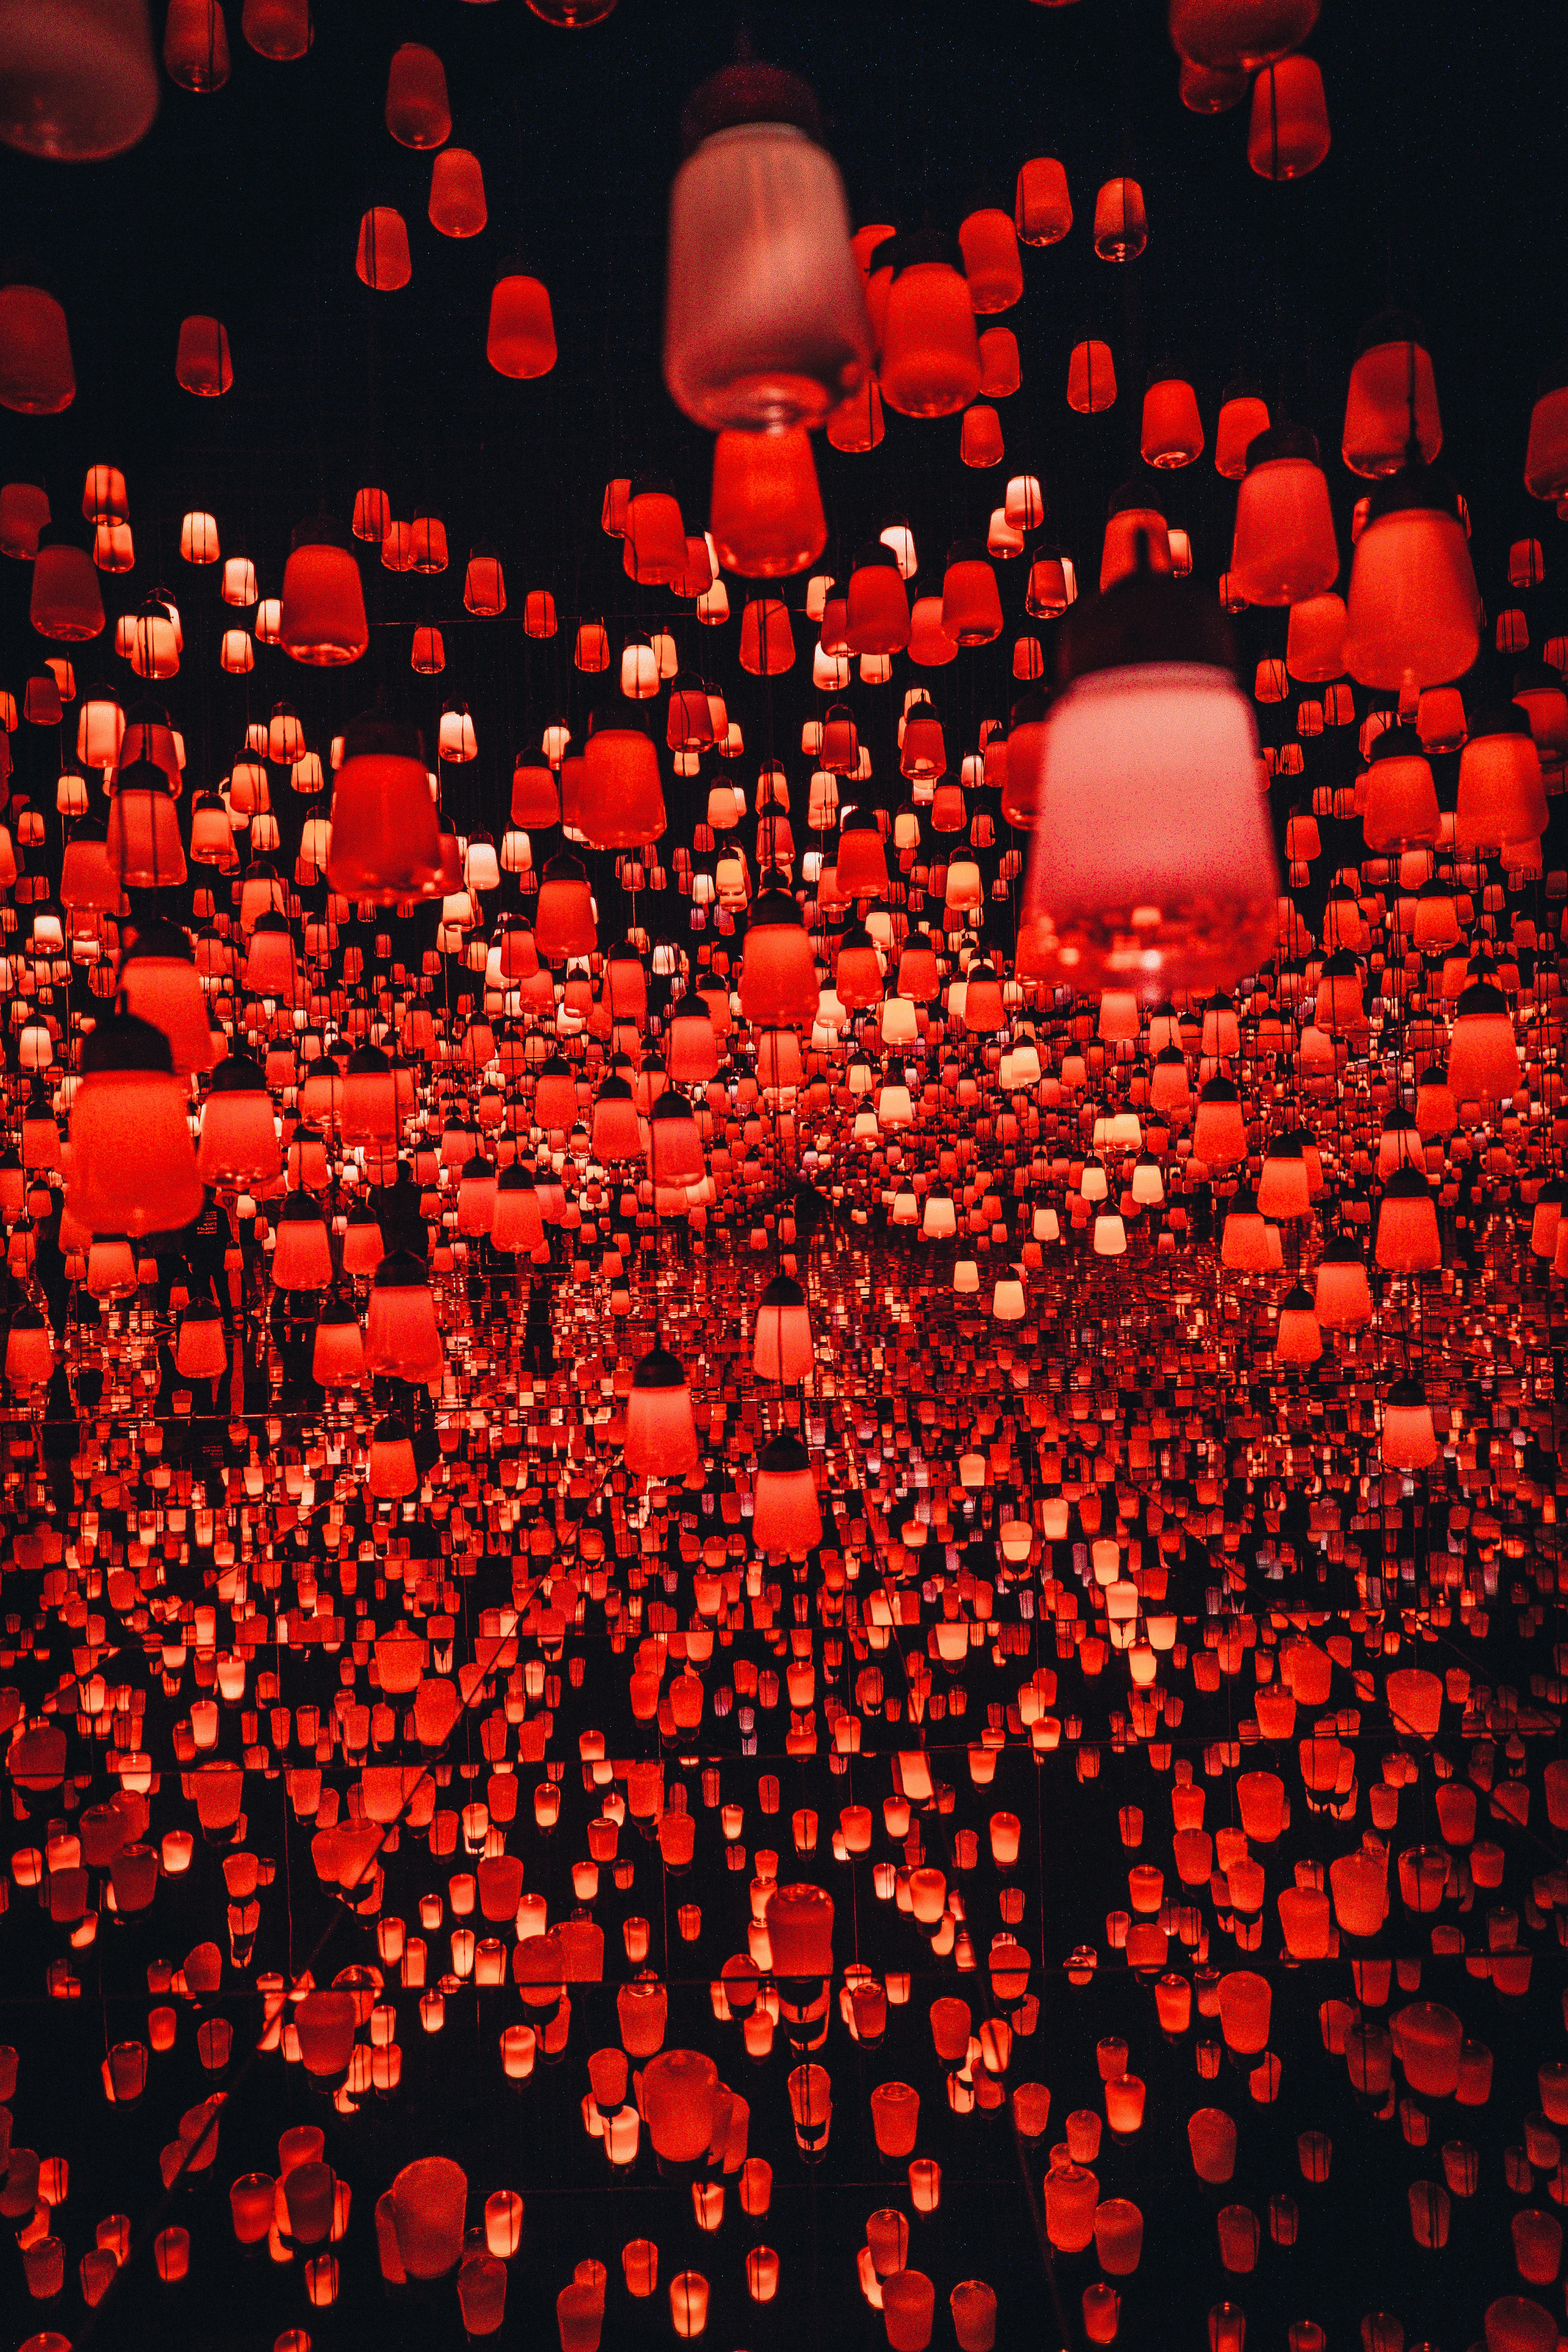
\includegraphics[width=6cm]{logo}}  %NEW: Changing logo
\def\extraspace{\vspace*{1.6cm}}
\makeatletter
\def\contactdetails{\faicon{phone} & \@telephone \\
                    \faicon{envelope} & \@email}
\makeatother

%%%% FRONT PAGE OF REPORTS

\def\reporttype{Report for}

\long\def\front#1#2#3{
\newpage
\begin{singlespacing}
\thispagestyle{empty}
\vspace*{-1.4cm}
\hspace*{-1.4cm}
\hbox to 16cm{
  \hbox to 6.5cm{\vbox to 14cm{\vbox to 25cm{
    \logo
    \vfill
    \parbox{6.3cm}{\raggedright
      \sf\color[rgb]{0, 0.29, 0.55}    % NEW color -company info------------------------------------------------------------------------------------
      {\large\textbf{\name}}\par
      \vspace{.7cm}
      \tabcolsep=0.12cm\sf\small
      \begin{tabular}{@{}ll@{}}\contactdetails
      \end{tabular}
      \vspace*{0.3cm}\par
      ABN: \abn\par
    }
  }\vss}\hss}
  \hspace*{0.2cm}
  \hbox to 1cm{\vbox to 14cm{\rule{4pt}{26.8cm}\vss}\hss\hfill}  %NEW: Thicker vertical line -----------------------------------------------------
  \hbox to 10cm{\vbox to 14cm{\vbox to 25cm{   
      \vspace*{3cm}\sf\raggedright
      \parbox{11cm}{\sf\raggedright\baselineskip=1.2cm
         \fontsize{24.88}{30}\color[rgb]{0, 0.29, 0.55}\sf\textbf{#1}}   % NEW: title color blue ----------------------------------------------
      \par
      \vfill
      \large
      \vbox{\parskip=0.8cm #2}\par
      \vspace*{2cm}\par
      \reporttype\\[0.3cm]
      \hbox{#3}%\\[2cm]\
      \vspace*{1cm}
      {\large\sf\textbf{\Date~\Month~\Year}}
   }\vss}
  }}
\end{singlespacing}
\newpage
}

\makeatletter
\def\titlepage{\front{\expandafter{\@title}}{\@author}{\@organization}}
\makeatother

\usepackage{setspace}
\setstretch{1.5}

%% Any special functions or other packages can be loaded here.
\usepackage{booktabs}
\usepackage{longtable}
\usepackage{array}
\usepackage{multirow}
\usepackage{wrapfig}
\usepackage{float}
\usepackage{colortbl}
\usepackage{pdflscape}
\usepackage{tabu}
\usepackage{threeparttable}
\usepackage{threeparttablex}
\usepackage[normalem]{ulem}
\usepackage{makecell}
\usepackage{xcolor}


\begin{document}           % Begining of document body -----------------------------------------------
\titlepage

{
\setcounter{tocdepth}{2}
\tableofcontents
}
\begin{Shaded}
\begin{Highlighting}[]
\NormalTok{knitr}\OperatorTok{::}\NormalTok{opts_chunk}\OperatorTok{$}\KeywordTok{set}\NormalTok{(}\DataTypeTok{echo =} \OtherTok{FALSE}\NormalTok{, }
                      \DataTypeTok{cache=}\OtherTok{TRUE}\NormalTok{, }
                      \DataTypeTok{messages=}\OtherTok{FALSE}\NormalTok{,}
                      \DataTypeTok{warning=}\OtherTok{FALSE}\NormalTok{)}
\end{Highlighting}
\end{Shaded}

\begin{verbatim}
## Parsed with column specification:
## cols(
##   .default = col_character(),
##   X = col_double(),
##   Y = col_double(),
##   reportedTime = col_double(),
##   beginTime = col_double(),
##   centergbsid = col_double(),
##   centerLong = col_double(),
##   centerLat = col_double(),
##   centerX = col_double(),
##   centerY = col_double(),
##   OBJECTID = col_double()
## )
\end{verbatim}

\begin{verbatim}
## See spec(...) for full column specifications.
\end{verbatim}

\begin{verbatim}
## OGR data source with driver: ESRI Shapefile 
## Source: "/Users/emsheehan/Documents/UNI - POSTGRAD/COLLAB/ETC5513-Assignment-4/data/Police_Incidents_Last_2Years-shp/Police_Incidents_Last_2Years.shp", layer: "Police_Incidents_Last_2Years"
## with 43283 features
## It has 0 fields
\end{verbatim}

\begin{verbatim}
## Parsed with column specification:
## cols(
##   .default = col_character(),
##   X = col_double(),
##   Y = col_double(),
##   PoliceUseOfForceID = col_double(),
##   ForceReportNumber = col_double(),
##   SubjectRoleNumber = col_double(),
##   EventAge = col_double(),
##   TotalCityCallsForYear = col_double(),
##   TotalPrecinctCallsForYear = col_double(),
##   TotalNeighborhoodCallsForYear = col_double(),
##   CenterGBSID = col_double(),
##   CenterLatitude = col_double(),
##   CenterLongitude = col_double(),
##   CenterX = col_double(),
##   CenterY = col_double(),
##   OBJECTID = col_double()
## )
\end{verbatim}

\begin{verbatim}
## See spec(...) for full column specifications.
\end{verbatim}

\hypertarget{introduction}{%
\section{Introduction}\label{introduction}}

George Floyd was arrested and killed by Derek Chauvin, a U.S. police officer, on the 25th of May in Minneapolis, \textcite{BBC-News-2020}. Chauvin knelt on George Floyd's neck for eight minutes and 46 seconds as Floyd gasped for air. His abominable death has sparked outrage on police brutality across America.

For several years, African-Americans have been the subject of racial vilification. In a study by \textcite{Dottolo-2008} students were interviewed and asked about police harassment and crime. Close analysis revealed that the students had stereotyped the criminals to be poor African American men. Another study by \ldots{} revealed

This paper hopes to explore and understand crime in Minneapolis. Specifically, the areas where crime is most common, the ethnicity of those committing the crime, and the force used by police.

\hypertarget{data}{%
\section{Data}\label{data}}

To perform this analysis data was downloaded from the City of \textcite{Minneapolis-2020}. The data obtained included the shapefiles, the crime dashboard (crime incident data) and the use of force dashboard (the use of force data).

The crime incident data had a high number of NA's, where the race of the offender was not recorded. To mitigate the impact on the calculated proportions, particularly where race is concerned, they were not removed. Unfortunately, this considered, the analysis will still be impacted and the resulting proportions may be over or under-estimated as a result of the missing values.

More limitations\ldots{}

\hypertarget{methodology}{%
\section{Methodology}\label{methodology}}

\hypertarget{analysing-the-crime-incidence}{%
\subsection{Analysing the Crime Incidence}\label{analysing-the-crime-incidence}}

\hypertarget{analysing-the-neighborhoods-with-the-most-crime}{%
\subsection{Analysing the Neighborhoods with the Most Crime}\label{analysing-the-neighborhoods-with-the-most-crime}}

\hypertarget{analysing-the-crime-over-time}{%
\subsection{Analysing the Crime over Time}\label{analysing-the-crime-over-time}}

\hypertarget{analysing-the-force-used-by-police}{%
\subsection{Analysing the Force Used by Police}\label{analysing-the-force-used-by-police}}

\hypertarget{mapping-the-use-of-force-data}{%
\subsection{Mapping the Use of Force Data}\label{mapping-the-use-of-force-data}}

\hypertarget{results}{%
\section{Results}\label{results}}

\hypertarget{crime-incidence}{%
\subsection{Crime Incidence}\label{crime-incidence}}

Figure \ref{fig:plot-number-crimes} demonstrates that across all years, theft is the most commonly committed crime in Minneapolis. In this instance theft includes; automobile theft, bike theft, coin-operated device theft, gas-station drive off, online theft, petty theft, pocket picking, scrapping-recycling theft, theft from a building, theft from a motor vehicle, theft from a person, other theft, theft by swindle and theft of motor vehicle parts. Burglary and assault are the second and third highest committed crimes, respectively. It should be noted that 2019 is the only complete year, hence the higher incidence.

\begin{figure}
\centering
\includegraphics{Assignment4_files/figure-latex/plot-number-crimes-1.pdf}
\caption{\label{fig:plot-number-crimes}Crime incidence according to Year and Offense Type}
\end{figure}

\hypertarget{neighborhoods-with-the-most-crimes}{%
\subsection{Neighborhoods with the Most Crimes}\label{neighborhoods-with-the-most-crimes}}

Figure \ref{fig:offencetype} captures the top five most frequent offenses in the neighborhoods with the highest crime rates. It is clear that theft is the most commonly committed crime across all neighborhoods, consistent with Figure \ref{fig:plot-number-crimes}. Comparitively, Longflow has a similar incidence of shoplifting and theft.

\begin{figure}

{\centering \includegraphics{Assignment4_files/figure-latex/offencetype-1} 

}

\caption{The most common offence type in the Neighborhoods with the highest Crime Incidence}\label{fig:offencetype}
\end{figure}

\begin{verbatim}
## Selecting by case
\end{verbatim}

\begin{table}

\caption{\label{tab:neighborhood-2018}Top 20 Neighborhoods with the Highest Crime Rate for 2018}
\centering
\begin{tabular}[t]{l|r}
\hline
neighborhood & case\\
\hline
CARAG & 194\\
\hline
Cedar Riverside & 225\\
\hline
Downtown West & 1199\\
\hline
East Phillips & 250\\
\hline
Elliot Park & 251\\
\hline
Folwell & 191\\
\hline
Hawthorne & 310\\
\hline
Jordan & 305\\
\hline
Longfellow & 378\\
\hline
Loring Park & 254\\
\hline
Lowry Hill East & 381\\
\hline
Marcy Holmes & 398\\
\hline
Near - North & 254\\
\hline
North Loop & 235\\
\hline
Powderhorn Park & 227\\
\hline
Prospect Park - East River Road & 246\\
\hline
Seward & 274\\
\hline
Ventura Village & 259\\
\hline
Whittier & 490\\
\hline
Willard - Hay & 221\\
\hline
\end{tabular}
\end{table}

\begin{verbatim}
## Selecting by case
\end{verbatim}

\begin{table}

\caption{\label{tab:neighborhood-2019}Top 20 Neighborhoods with the Highest Crime Rate for 2019}
\centering
\begin{tabular}[t]{l|r}
\hline
neighborhood & case\\
\hline
Cedar Riverside & 398\\
\hline
Downtown West & 2612\\
\hline
East Phillips & 439\\
\hline
Elliot Park & 508\\
\hline
Folwell & 363\\
\hline
Hawthorne & 578\\
\hline
Jordan & 483\\
\hline
Longfellow & 768\\
\hline
Loring Park & 515\\
\hline
Lowry Hill East & 817\\
\hline
Marcy Holmes & 726\\
\hline
Midtown Phillips & 490\\
\hline
Near - North & 506\\
\hline
North Loop & 470\\
\hline
Powderhorn Park & 460\\
\hline
Prospect Park - East River Road & 414\\
\hline
Seward & 553\\
\hline
Ventura Village & 516\\
\hline
Whittier & 1182\\
\hline
Willard - Hay & 369\\
\hline
\end{tabular}
\end{table}

\begin{verbatim}
## Selecting by case
\end{verbatim}

\begin{table}

\caption{\label{tab:neighborhood-2020}Top 20 Neighborhoods with the Highest Crime Rate for 2020}
\centering
\begin{tabular}[t]{l|r}
\hline
neighborhood & case\\
\hline
CARAG & 139\\
\hline
Cedar Riverside & 140\\
\hline
Downtown West & 589\\
\hline
East Phillips & 185\\
\hline
Elliot Park & 159\\
\hline
Hawthorne & 177\\
\hline
Jordan & 200\\
\hline
Longfellow & 274\\
\hline
Loring Park & 209\\
\hline
Lowry Hill East & 268\\
\hline
Marcy Holmes & 271\\
\hline
Midtown Phillips & 174\\
\hline
Near - North & 215\\
\hline
North Loop & 195\\
\hline
Powderhorn Park & 155\\
\hline
Prospect Park - East River Road & 150\\
\hline
Seward & 216\\
\hline
Ventura Village & 237\\
\hline
Whittier & 415\\
\hline
Willard - Hay & 146\\
\hline
\end{tabular}
\end{table}

\begin{figure}
\centering
\includegraphics{Assignment4_files/figure-latex/neighborhood2018-1.pdf}
\caption{\label{fig:neighborhood2018}Top 20 Neighborhoods with the Highest Crime Rate for 2018}
\end{figure}

\begin{figure}
\centering
\includegraphics{Assignment4_files/figure-latex/neighborhood2019-1.pdf}
\caption{\label{fig:neighborhood2019}Top 20 Neighborhoods with the Highest Crime Rate for 2019}
\end{figure}

\begin{figure}
\centering
\includegraphics{Assignment4_files/figure-latex/neighborhood2020-1.pdf}
\caption{\label{fig:neighborhood2020}Top 20 Neighborhoods with the Highest Crime Rate for 2020}
\end{figure}

Figure \ref{fig:neighborhood2018}, Figure \ref{fig:neighborhood2019} and Figure \ref{fig:neighborhood2020}, show that across all years \textbf{Downtown West} and \textbf{Whittier} have the highest crime rate, followed by \textbf{Longfellow}, \textbf{Lowry Hill East} and \textbf{Marcy Holmes}.

Figure \ref{fig:Crimeanalysis} explores the relationship between precinct and offense type. Across all precincts, theft is the most commonly committed crime, consistent with Figure \ref{fig:plot-number-crimes}. Interestingly enough, precinct 1 and 2 have a similar incidence of theft, however, precinct 5 has a much higher incidence of bulglary.

\begin{figure}

{\centering \includegraphics{Assignment4_files/figure-latex/Crimeanalysis-1} 

}

\caption{Crimes comparison of different districts}\label{fig:Crimeanalysis}
\end{figure}

\hypertarget{crime-over-time}{%
\subsection{Crime over Time}\label{crime-over-time}}

Figure \ref{fig:timefig} compares the incidence of crimes in each month. As stated above, 2019 is the only complete year in the data set. In 2018, crime peaked in October, and dropped in December. In 2019, crime was very low in the colder months (January, February and March), peaking in the summer months (July and August). Comparitively, the incidence of crime in 2020 was much lower than 2019 and did not increase in May, which is likely due to the stay at home orders resulting from COVID-19.

\begin{figure}

{\centering \includegraphics{Assignment4_files/figure-latex/timefig-1} 

}

\caption{Comparison of crimes in different months}\label{fig:timefig}
\end{figure}

\hypertarget{force-used-by-police-data}{%
\subsection{Force Used by Police Data}\label{force-used-by-police-data}}

Figure \ref{fig:weekdaysituation} show the distribution of crime and force used over a given week. There are more crimes on weekdays than on weekends, however, the force use by police is the opposite with greater force use on weekends. It is likely that weekends will attract larger crowds, particularly at entertainment venues, therefore attracting a larger police presence. Furthermore, it is unlikely criminals will commit crimes, particularly when police presence is so high.

\begin{figure}

{\centering \includegraphics{Assignment4_files/figure-latex/weekdaysituation-1} 

}

\caption{The average crimes and force using in a week}\label{fig:weekdaysituation}
\end{figure}

Figure \ref{fig:TypeOfResistance} shows the resistance used in each precinct. In essence, this figure captures the prevalance of crime and perhaps the effiency of police in controlling the crime rate. It can be inferred that the fourth precinct is significantly more dangerous than the fifth precinct, and the force use in the fourth precinct is much higher.

\begin{figure}

{\centering \includegraphics{Assignment4_files/figure-latex/TypeOfResistance-1} 

}

\caption{The different Resistance of criminals in each Precinct}\label{fig:TypeOfResistance}
\end{figure}

Figure \ref{fig:relationshipfig} shows the relationship between the force type and the type of resistance. This figure captures the effectiveness of the force type used by police. If the only resistance used by police is a dog, criminals are more likely to flee on foot. However, if a firearm or chemical irritant is used, criminals are less likely to escape.

\begin{figure}

{\centering \includegraphics{Assignment4_files/figure-latex/relationshipfig-1} 

}

\caption{The relationship between Force Type adopted by police and type of resistance of criminals}\label{fig:relationshipfig}
\end{figure}

Figure \ref{fig:Race} shows the use of force, according to race. It is clear that African Americans are subject to more aggressive forms of force. Further, the figure demonstrates police are less likely to use less lethal force on African Americans.

\begin{figure}

{\centering \includegraphics{Assignment4_files/figure-latex/Race-1} 

}

\caption{Different races are treated differently}\label{fig:Race}
\end{figure}

\clearpage

\hypertarget{police-use-of-force-map-analysis}{%
\section{Police use of force map analysis}\label{police-use-of-force-map-analysis}}

\begin{figure}
\centering
\includegraphics{Assignment4_files/figure-latex/puofbar-1.pdf}
\caption{\label{fig:puofbar}proportion of race in police use of force by Precincts}
\end{figure}

Dataset comes from \textcite{openmn}
\textbf{Figure \ref{fig:puofbar}} shows the proportion of race in police use of force by Precincts.

\begin{quote}
WIP: need to join table with demographics (racial composition in each Precinct) and data on proportion of crimes commited by race in each precinct.
\end{quote}

\hypertarget{police-use-of-force-map}{%
\subsection{Police use of force map}\label{police-use-of-force-map}}

\begin{verbatim}
## OGR data source with driver: ESRI Shapefile 
## Source: "/Users/emsheehan/Documents/UNI - POSTGRAD/COLLAB/ETC5513-Assignment-4/data/Police_Use_of_Force-shp/Police_Use_of_Force.shp", layer: "Police_Use_of_Force"
## with 30024 features
## It has 28 fields
\end{verbatim}

\begin{verbatim}
## Reading layer `Police_Use_of_Force' from data source `/Users/emsheehan/Documents/UNI - POSTGRAD/COLLAB/ETC5513-Assignment-4/data/Police_Use_of_Force-shp/Police_Use_of_Force.shp' using driver `ESRI Shapefile'
## Simple feature collection with 30024 features and 28 fields
## geometry type:  POINT
## dimension:      XY
## bbox:           xmin: -93.32842 ymin: 0 xmax: 0 ymax: 45.05124
## CRS:            4326
\end{verbatim}

\begin{figure}

{\centering \includegraphics{Assignment4_files/figure-latex/puofmap-1} 

}

\caption{Number of police use of force incidents in Precincts}\label{fig:puofmap}
\end{figure}

\textbf{Figure \ref{fig:puofmap}} shows the police use of force map in Minneapolis. The numbers show number of incidents per precinct.

\hypertarget{precincts}{%
\subsection{Precincts}\label{precincts}}

\includegraphics{Assignment4_files/figure-latex/unnamed-chunk-3-1.pdf}

\printbibliography

\end{document}

